\documentclass{beamer}
\usepackage[utf8]{inputenc}
\usepackage{tikz}
\usetikzlibrary{arrows.meta}
\tikzset{>={Latex[width=2mm,length=2mm]},
  base/.style = {
    rectangle, rounded corners, draw=black,
    minimum height=1cm, text centered, font=\sffamily
  },
  process/.style = {
    base, minimum width=2.5cm, fill=orange!15,
    font=\ttfamily
  },
}

\graphicspath{{./img/}}
\DeclareGraphicsExtensions{.png,.jpg,.pdf}

\usepackage{hyperref}
\hypersetup{colorlinks,urlcolor=blue!50!black,linkcolor=red}

\usepackage{fontawesome}
\usepackage{listings}

\title{\small Máster en Sistemas Electrónicos Avanzados (MSEA)\\\Large Co-simulación y verificación funcional con\\VHDL, C/C++ y Python/m}
\author{Unai Martinez Corral\\\href{mailto:unai.martinezcorral@ehu.eus}{\faEnvelope~unai.martinezcorral@ehu.eus} ~\href{https://github.com/umarcor}{\faGithub~umarcor}}
\institute{Dpto. Tecnología Electrónica\\Grupo de Investigación de Diseño en Electrónica Digital (GDED)\\Escuela de Ingeniería de Bilbao\\Universidad del País Vasco/Euskal Herriko Unibertsitatea (UPV/EHU)}
\date{2020/03}

\begin{document}

\frame{\titlepage}

\begin{frame}
\frametitle{Languages}
\vfill
\small
\begin{minipage}[t]{.49\linewidth}
\begin{itemize}
\item Dynamic/static
\item Interpreted/compiled
\item Strong/loose typing
\item Runtime
\item Memory management (GC)
\item Concurrency/parallelism
\end{itemize}
\end{minipage}
\begin{minipage}[t]{.5\linewidth}
\begin{itemize}
\item Assembly/ASM
\item Ada, C/C++, Java, C\#
\item go(lang), Rust
\item Python, m, Julia, Perl, Ruby
\item JavaScript, TypeScript
\item shell/bash, powershell, cmd
\item LaTeX/Tikz
\item MarkDown, reStructuredText
\item HTML, CSS/SASS
\item \ldots
\end{itemize}
\end{minipage}
\vfill
\centering
\href{https://en.wikipedia.org/wiki/Comparison_of_programming_languages}{\faWikipediaW~Comparison of programming languages}
\end{frame}

\begin{frame}
\frametitle{Languages: compilation and execution}
\centering
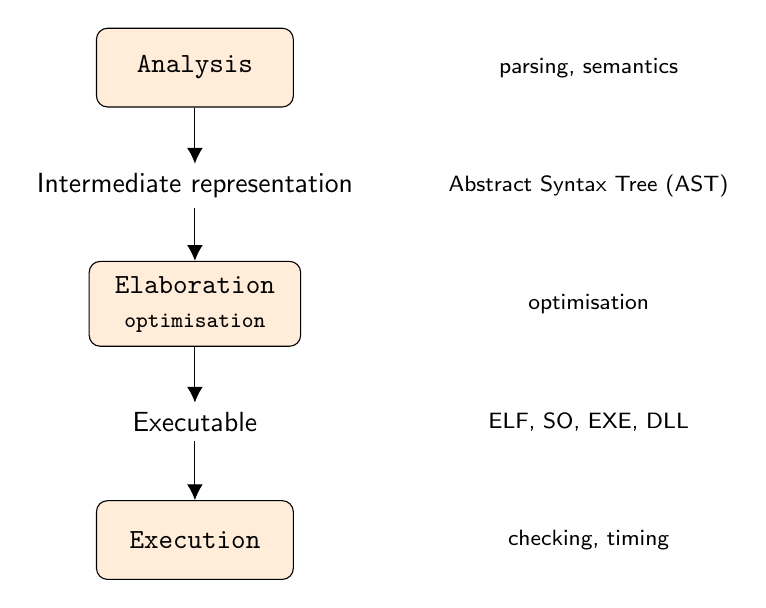
\begin{tikzpicture}[node distance=1.5cm, every node/.style={fill=white, font=\sffamily}]
  \node (ana) [process] {Analysis};
  \node (ana_i) [right of=ana, node distance=5cm] {\footnotesize parsing, semantics};
  \node (ast) [below of=ana] {Intermediate representation};
  \node (ast_i) [right of=ast, node distance=5cm] {\footnotesize Abstract Syntax Tree (AST)};
  \node (ela) [process, below of=ast] {\begin{tabular}{c}Elaboration\\\footnotesize optimisation\end{tabular}};
  \node (ela_i) [right of=ela, node distance=5cm] {\footnotesize optimisation};
  \node (bin) [below of=ela] {Executable};
  \node (bin_i) [right of=bin, node distance=5cm] {\footnotesize ELF, SO, EXE, DLL};
  \node (run) [process, below of=bin] {Execution};
  \node (run_i) [right of=run, node distance=5cm] {\footnotesize checking, timing};
  \draw[->] (ana) -- (ast);
  \draw[->] (ast) -- (ela);
  \draw[->] (ela) -- (bin);
  \draw[->] (bin) -- (run);
\end{tikzpicture}
\end{frame}

\begin{frame}
\frametitle{Languages: unified compilation tools}
\begin{itemize}
\item GNU Compiler Collection (GCC) \href{https://gcc.gnu.org/}{\faGlobe}
\item Low-level virtual machine (LLVM) \href{https://llvm.org/}{\faGlobe}; {\footnotesize despite its name, LLVM has little to do with traditional virtual machines.}
\end{itemize}
\vspace{1.5em}
\begin{itemize}
\item Java virtual machine (JVM) \href{https://en.wikipedia.org/wiki/Java_virtual_machine}{\faWikipediaW}
\item Dynamic Binary Modification/Translation (QEMU) \href{https://www.qemu.org/}{\faGlobe}
\item WebAssembly \href{https://webassembly.org/}{\faGlobe} \href{https://en.wikipedia.org/wiki/WebAssembly}{\faWikipediaW}
\end{itemize}
\end{frame}

\begin{frame}
\frametitle{IEEE Hardware Description Languages}
\vfill
\begin{itemize}
\item 1076: \textbf{VHDL} (1987, 1993, 2000, 2002, 2008, 2019)
\item 1076.1: \textbf{VHDL-AMS} (1999, 2007, 2017)
\item 1364: \textbf{Verilog} (1995, 2001 2005)
\item 1800: \textbf{SystemVerilog} (2005, 2009, 2012, 2017)
\item 1850: Property Specification Language (\textbf{PSL}) (2005, 2010)
\item 1666: \textbf{SystemC} (2005, 2011, 2016)
\end{itemize}
\vfill
\centering
\Large\href{https://standards.ieee.org}{\faGlobe~standards.ieee.org}
\end{frame}

\begin{frame}
\frametitle{HDL generators}
\begin{itemize}
\item High-Level Synthesis (HLS)
\href{https://en.wikipedia.org/wiki/High-level_synthesis}{\faWikipediaW}

\item Bluespec SystemVerilog (BSV) \href{https://bluespec.com/}{\faGlobe}
\href{https://github.com/bluespec}{\faGithub} \href{https://github.com/B-Lang-org/bsc}{\faGit}

\item Scala:
Chisel
\href{https://www.chisel-lang.org/}{\faGlobe} \href{https://github.com/freechipsproject/chisel3}{\faGithub},
SpinalHDL
\href{https://github.com/SpinalHDL}{\faGithub} \href{https://spinalhdl.github.io/SpinalDoc-RTD/}{\faBook}

\item Python:
MyHDL
\href{http://www.myhdl.org/}{\faGlobe} \href{https://github.com/myhdl/myhdl}{\faGithub},
Migen/nmigen
\href{https://m-labs.hk/gateware/migen/}{\faGlobe}
\href{https://github.com/m-labs?type=source}{\faGithub}
\item Haskell:
Clash
\href{https://clash-lang.org/}{\faGlobe}
\href{https://github.com/clash-lang}{\faGithub}

\item \ldots
\end{itemize}
\vspace{2em}
\begin{itemize}
\item Flexible Intermediate Representation for RTL (FIRRTL)
\href{https://github.com/freechipsproject/firrtl}{\faGithub}
\href{https://freechipsproject.github.io/firrtl/}{\faBook}
\end{itemize}
\end{frame}

\begin{frame}
\frametitle{HDL simulation}
\vfill
\begin{itemize}
\item Mentor Graphics/Siemens, Intel-Altera: ModelSim/QuestaSim
\item Aldec: Active-HDL/Riviera-PRO
\item Xilinx: ISE ISIM, Vivado XSIM
\item Cadence: Incisive
\item Synopsys: VCS
\end{itemize}
\vfill
\centering
\href{https://en.wikipedia.org/wiki/List_of_HDL_simulators}{\faWikipediaW~List of HDL simulators}
\end{frame}

\begin{frame}
\frametitle{Circuit simulation: open source}
\begin{minipage}[t]{.58\linewidth}
HDL simulation:
\begin{itemize}
\item GHDL
\href{https://github.com/ghdl/ghdl}{\faGithub}
\href{https://ghdl.rtfd.io}{\faBook}

\item nvc
\href{https://github.com/nickg/nvc}{\faGithub}

\item Verilator
\href{https://www.veripool.org/wiki/verilator}{\faGlobe}
\href{https://github.com/verilator/verilator}{\faGithub}

\item Icarus Verilog (iverilog)
\href{http://iverilog.icarus.com/}{\faGlobe}
\href{https://github.com/steveicarus/iverilog}{\faGithub}
\end{itemize}
\end{minipage}
\begin{minipage}[t]{.405\linewidth}
Analog simulation:
\begin{itemize}
\item Xyce \href{https://xyce.sandia.gov/}{\faGlobe} \href{https://github.com/Xyce/Xyce}{\faGithub}
\item SPICE \href{https://en.wikipedia.org/wiki/SPICE}{\faWikipediaW}
\item Ngspice \href{http://ngspice.sourceforge.net/}{\faGlobe}
\item Gnucap \href{http://gnucap.org}{\faGlobe}
\end{itemize}
\end{minipage}

\vfill
Waveform visualisation:
\begin{itemize}
\item GtkWave (LXT, LXT2, VZT, FST, GHW, VCD/EVCD)
\href{http://gtkwave.sourceforge.net/}{\faGlobe}
\href{https://github.com/gtkwave/gtkwave}{\faGithub}
\end{itemize}

\end{frame}

\begin{frame}
\frametitle{HDL simulation: GHDL}
\small Free and open-source  analyser, compiler, simulator and experimental synthesiser for VHDL. GHDL is not an interpreter: it allows to generate machine code from design sources.
\vspace{1em}
\begin{itemize}
  \item Full support for the 1987, 1993, 2002 versions of VHDL, and partial for 2008. Partial support of PSL.
  \item Three backends: LLVM, GCC or, x86\_64/i386 only, a built-in one (mcode).
  \item GNU/Linux, Windows and macOS; on x86, x86\_64, armv6/armv7/aarch32 and aarch64.
  \item Can write waveforms (GHW, VCD or FST).
  \item ghdl-ls implements Language Server Protocol (LSP) in Python.
  \item Synthesis: plain VHDL or yosys (through ghdlsynth).
\end{itemize}
\end{frame}

\begin{frame}
\frametitle{HDL co-simulation}
\begin{itemize}
  \item Verilog Procedural Interface (\textbf{VPI}), also known as Program Language Interface (\textbf{PLI}) 2.0.
\end{itemize}
\vspace{1em}
\begin{itemize}
  \item VHDL Procedural Interface (\textbf{VHPI}), or specific implementations, such as Foreign Language Interface (\textbf{FLI}).
\end{itemize}
\vspace{1em}
\begin{itemize}
  \item Generation of C/C++ models/sources through a transpiler.
\end{itemize}
\end{frame}

\begin{frame}
\frametitle{Functional verification of an HDL design}
\centering
\includegraphics[width=\linewidth]{cosim.pdf}
\end{frame}

\begin{frame}
\frametitle{Functional verification of a non-trivial HDL design}
\centering
\includegraphics[width=\linewidth]{cosim_zoom.pdf}
\end{frame}

\begin{frame}
\frametitle{VHDL simulation: libraries/frameworks for verification}
\begin{itemize}
\item UVM: Universal Verification Methodology \href{https://en.wikipedia.org/wiki/Universal_Verification_Methodology}{\faWikipediaW}
\vspace{.5em}

\item OSVVM: Open Source VHDL Verification Methodolody
\href{https://osvvm.org/}{\faGlobe}
\href{https://github.com/OSVVM/OSVVM}{\faGithub}
\vspace{.5em}

\item UVVM: Universal VHDL Verification Methodology \href{https://bitvis.no/dev-tools/uvvm/}{\faGlobe}
\href{https://github.com/UVVM}{\faGithub}
\vspace{2em}

\item cocotb: Coroutine Co-simulation Test Bench
\href{https://github.com/cocotb/cocotb}{\faGithub}
\href{https://cocotb.rtfd.io}{\faBook}
\href{http://potential.ventures/cocotb}{\faGlobe}
\href{https://pypi.org/project/cocotb/}{\faCode}
\vspace{.5em}

\item VUnit: unit testing framework
\href{https://github.com/VUnit/vunit}{\faGithub}
\href{http://vunit.github.io/}{\faBook}
\href{https://pypi.org/project/vunit-hdl/}{\faCode}

\begin{itemize}
\item VUnit/cosim
\href{https://github.com/VUnit/cosim}{\faGithub}
\href{https://vunit.github.io/cosim/}{\faBook}
\end{itemize}
\end{itemize}
\end{frame}

\begin{frame}
\frametitle{HDL simulation: VUnit}
\small
Open source unit testing framework for VHDL/SystemVerilog. It features the functionality needed to realize continuous and automated testing of your HDL code. VUnit complements traditional testing methodologies by supporting a \emph{test early and often} approach through automation.
\vspace{1em}
\begin{itemize}
  \item Supported languages: VHDL (93, 2002, 2008, 2019), Verilog, SystemVerilog
  \item Supported simulators: GHDL, Aldec Riviera-PRO/Active-HDL, Mentor Graphics ModelSim/Questa and Cadence Incisive (experimental)
  \item Requires Python $>=3.6$: Python Interface and CLI
  \item Supported on Windows, GNU/Linux and macOS.
  \item VHDL libraries: OSVVM, JSON-for-VHDL, Run, Check, Logging, Communication, Verification Components, etc.
  \item Data Types with an external API for co-simulation
\end{itemize}
\end{frame}

\begin{frame}
\frametitle{VUnit: overview}
\centering
\includegraphics[width=\linewidth]{vunit_cosim.pdf}
\end{frame}

\begin{frame}
\frametitle{Work environment}
\begin{itemize}
  \item GHDL (LLVM or GCC backends)
  \vspace{1em}

  \item Python $>=3.6$
  \vspace{1em}

  \item Editor: Visual Studio Code (VSC), vim, emacs, Sigasi...
  \vspace{1em}

  \item GtkWave
  \vspace{1em}

  \item Language server: ghdl-ls, rust\_hdl...
\end{itemize}
\end{frame}

\begin{frame}
\frametitle{Exercises: introduction}
GHDL Quick Start Guide \href{https://ghdl.readthedocs.io/en/latest/examples/quick_start/README.html}{\faBook}
\vspace{1em}
\begin{itemize}
  \item Hello World
  \href{https://ghdl.readthedocs.io/en/latest/examples/quick_start/hello/README.html}{\faBook}
  \vspace{1em}

  \item Heartbeat
  \href{https://ghdl.readthedocs.io/en/latest/examples/quick_start/heartbeat/README.html}{\faBook}
  \vspace{1em}

  \item Full-adder
  \href{https://ghdl.readthedocs.io/en/latest/examples/quick_start/adder/README.html}{\faBook}
\end{itemize}
\vspace{2em}

VUnit User Guide \href{http://vunit.github.io/user_guide.html}{\faBook}
\vspace{1em}
\begin{itemize}
  \item Add \lstinline{run.py} to Full-adder
\end{itemize}
\end{frame}

\begin{frame}
\frametitle{VUnit: tutorial}
\centering
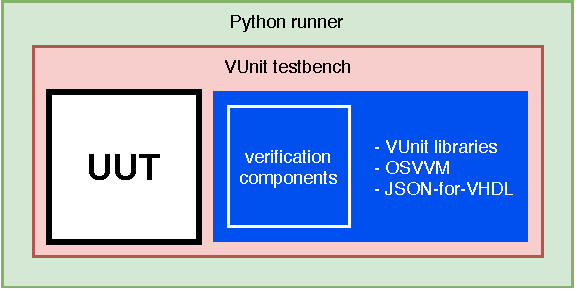
\includegraphics[width=\linewidth]{vunit_overview.pdf}
\end{frame}

\begin{frame}
\frametitle{Exercises: libraries}
\begin{itemize}
  \item Run
  \href{http://vunit.github.io/run/user_guide.html}{\faBook}
  \href{https://github.com/VUnit/vunit/tree/master/examples/vhdl/run}{\faCode}
  \vspace{.5em}

  \item Logging
  \href{http://vunit.github.io/logging/user_guide.html}{\faBook}
  \href{https://github.com/VUnit/vunit/tree/master/examples/vhdl/logging}{\faCode}
  \vspace{.5em}

  \item Check
  \href{http://vunit.github.io/check/user_guide.html}{\faBook}
  \href{https://github.com/VUnit/vunit/tree/master/examples/vhdl/check}{\faCode}
  \vspace{.5em}

  \item Communication
  \href{http://vunit.github.io/com/user_guide.html}{\faBook}
  \href{https://github.com/VUnit/vunit/tree/master/examples/vhdl/com/}{\faCode}
  \vspace{1em}

  \item OSVVM
  \begin{itemize}
    \item array
    \href{https://github.com/VUnit/vunit/tree/master/examples/vhdl/array}{\faCode}
  \end{itemize}
  \vspace{.5em}

  \item JSON-for-VHDL
  \begin{itemize}
    \item json4vhdl
    \href{https://github.com/VUnit/vunit/tree/master/examples/vhdl/json4vhdl}{\faCode}
    \item composite\_generics
    \href{https://github.com/VUnit/vunit/tree/master/examples/vhdl/composite_generics}{\faCode}
  \end{itemize}
  \vspace{1em}
\end{itemize}

\end{frame}

\begin{frame}
\frametitle{Exercises: verification components}
Verification Component Library (VCL) \href{http://vunit.github.io/verification_components/user_guide.html}{\faBook}
\vspace{1em}
\begin{itemize}
  \item uart
  \href{https://github.com/VUnit/vunit/tree/master/examples/vhdl/uart}{\faCode}
  \vspace{1em}

  \item array\_axis\_vcs
  \href{https://github.com/VUnit/vunit/tree/master/examples/vhdl/array_axis_vcs}{\faCode}
  \vspace{1em}

  \item axi\_dma
  \href{https://github.com/VUnit/vunit/tree/master/examples/vhdl/axi_dma}{\faCode}
\end{itemize}
\end{frame}

\begin{frame}
\frametitle{Exercises: co-simulation}
VUnit External VHDL API \href{http://vunit.github.io/data_types/user_guide.html\#external-vhdl-api}{\faBook}
\vspace{1em}

VUnit/cosim \href{https://vunit.github.io/cosim}{\faBook}
\vspace{1em}
\begin{itemize}
  \item copy
  \href{https://vunit.github.io/cosim/examples/copy.html}{\faBook}
  \href{https://github.com/VUnit/cosim/tree/master/examples/copy}{\faCode}
  \vspace{1em}

  \item buffer
  \href{https://vunit.github.io/cosim/examples/buffer.html}{\faBook}
  \href{https://github.com/VUnit/cosim/tree/master/examples/buffer}{\faCode}
\end{itemize}
\end{frame}

\begin{frame}
\frametitle{Exercises: AXIS co-simulation}
\centering
\includegraphics[width=.8\linewidth]{vunit_axiscosim.pdf}
\end{frame}

\begin{frame}
\frametitle{Dynamic Binary Hardware Injection (DBHI)}
\centering
\includegraphics[width=\linewidth]{diagram.pdf}

\vfill
\Large\href{https://dbhi.github.io/}{dbhi.github.io}
\end{frame}

\begin{frame}
\frametitle{Other open source projects}
\begin{minipage}[t]{.495\linewidth}
Project management:
\begin{itemize}
  \item tsfpga
  \href{https://gitlab.com/truestream/tsfpga}{\faGit} \href{https://truestream.gitlab.io/tsfpga/}{\faBook}
  \href{https://pypi.org/project/tsfpga/}{\faCode}

  \item fusesoc
  \href{https://github.com/olofk/fusesoc}{\faGithub}
  \href{https://fusesoc.rtfd.io/}{\faBook}
  \href{https://pypi.org/project/fusesoc/}{\faCode}

  \item edalize
  \href{https://github.com/olofk/edalize}{\faGithub}
  \href{https://edalize.rtfd.io}{\faBook}
  \href{https://pypi.org/project/edalize/}{\faCode}

  \item litex
  \href{https://github.com/enjoy-digital/litex}{\faGithub}

  \item duh
  \href{https://github.com/sifive/duh}{\faGithub}
\end{itemize}
\vspace{1em}

Waveform viewer/drawer:
\begin{itemize}
  \item wavedrom
  \href{https://github.com/wavedrom/wavedrom}{\faGithub}
  \href{https://wavedrom.com/}{\faGlobe}
\end{itemize}
\end{minipage}
\begin{minipage}[t]{.49\linewidth}
Android:
\begin{itemize}
  \item termux \href{https://termux.com/}{\faGlobe} \href{https://github.com/termux}{\faGithub}
  \begin{itemize}
      \item gcc\_termux \href{https://github.com/its-pointless/gcc_termux}{\faGithub}
  \end{itemize}
\end{itemize}
\vspace{1em}

Formal verification:
\begin{itemize}
  \item ghdlsynth-beta
  \href{https://github.com/tgingold/ghdlsynth-beta}{\faGithub}

  \item yosys
  \href{https://github.com/YosysHQ/yosys}{\faGithub}
  \href{http://www.clifford.at/yosys/}{\faGlobe}

  \item nextpnr
  \href{https://github.com/YosysHQ/nextpnr}{\faGithub}

  \item SymbiYosys
  \href{https://github.com/YosysHQ/SymbiYosys}{\faGithub}
  \href{https://symbiyosys.rtfd.io}{\faBook}
\end{itemize}
\end{minipage}
\end{frame}

\begin{frame}
\frametitle{SymbiFlow}
\centering
\includegraphics[width=\linewidth]{symbiflow.png}
\vfill
\Large\href{https://symbiflow.github.io/}{symbiflow.github.io}
\end{frame}

\end{document}

